\section{Preprocessing Ablation}
\label{sec:ablation}

RQ3 asks how much preprocessing matters. We vary one factor at a time, holding
model, features, split and tuning budget fixed; the contrast is scaling, with P0
unscaled and P2 standardised on training rows only.

% GENERATED by scripts/build_latex_assets.py -- do not edit by hand.
\begin{table}[t]
\centering
\caption{Controlled preprocessing ablation: validation MAE without standardisation (P0) and with it (P2), holding model, features, split and tuning budget fixed. A change of exactly $0.000\%$ means the model is invariant to monotone per-feature rescaling, which is the theoretical prediction for tree ensembles and serves as a negative control.}
\label{tab:ablation}
\small
\setlength{\tabcolsep}{4pt}
\begin{tabular}{@{}l r r r r r@{}}
\toprule
 & \multicolumn{3}{c}{AAPL} & \multicolumn{2}{c}{BTC} \\
\cmidrule(lr){2-4}\cmidrule(l){5-6}
Model & P0 MAE & P2 MAE & $\Delta$ & P0 MAE & $\Delta$ \\
\midrule
Linear baseline & 2.899 & 2.920 & +0.745 & 1600.205 & +0.211 \\
Ridge & 2.898 & 2.897 & -0.041 & 1601.874 & +0.032 \\
SVR (RBF) & 2.891 & 2.890 & -0.010 & 1604.186 & -0.066 \\
Random forest & 2.928 & 2.928 & \textbf{0.000} & 1603.373 & \textbf{0.000} \\
Hist.\ gradient boosting & 2.898 & 2.898 & \textbf{0.000} & 1605.016 & \textbf{0.000} \\
\bottomrule
\end{tabular}
\par\smallskip\footnotesize
$\Delta$ is the percentage change in validation MAE from P0 to P2. Bold $0.000$ denotes bit-identical predictions.
\end{table}


The measured pattern matches Section~\ref{sec:background}, exactly rather than
approximately: for both tree ensembles the change in validation MAE is
\emph{bit-identical} --- $0.000\%$ to printed precision --- on both assets. That is a strong internal control: had scaling moved the forests, the correct
inference would be a bug, not a discovery.

Scaling-sensitive families move slightly and not uniformly helpfully:
standardisation barely changes AAPL Ridge, worsens the AAPL linear baseline
(Table~\ref{tab:ablation}) and rescues nothing --- every value stays within about
one percentage point of the baseline. An ablation ending in no
substantial effect is a legitimate finding, and a useful teaching one: it
separates \emph{this transform changes the model} from \emph{this transform
improves the forecast}.

One variant is reported as not run: with no missing values in either snapshot an
imputation variant would duplicate the baseline cell, and we did not inject
synthetic gaps to manufacture a contrast.

\begin{figure}[t]
  \centering
  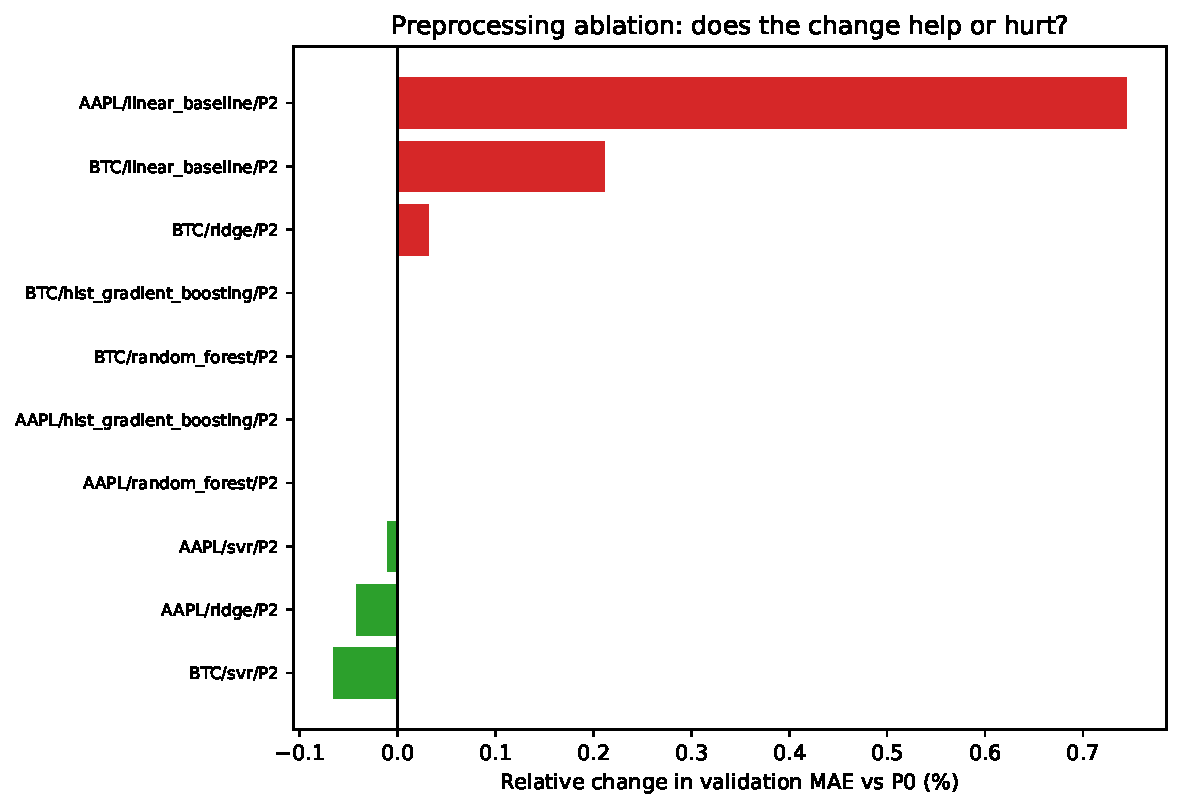
\includegraphics[width=\linewidth]{figures/fig06_ablation_delta.pdf}
  \caption{Relative change in validation MAE between unscaled (P0) and
  standardised (P2) variants, holding model and asset fixed. Bars at exactly zero
  are the tree ensembles, whose predictions are bit-identical under monotone
  rescaling. Only matched cells are plotted.}
  \label{fig:ablation}
\end{figure}
